%!TEX root = ../dokumentation.tex

\chapter{Grundlagen}

\section{JavaScript}

\subsection{Der Sprachstandard ECMAScript}\label{sec:der-sprachstandard-ecmascript}
ECMAScript spezifiziert den Sprachstandard von JavaScript. Dieser wird seit dem Jahr 1997 Jahren von der European Computer Manufactures Association (kurz: ECMA) weiterentwickelt. Zunächst wurden die Versionen durchnummeriert (ES1, ES2, ES3, ES4, und ES5). Im Jahre 2015 wurde beschlossen, dass jährlich eine neue Version von ECMAScript erscheinen soll. Daher tragen die nachfolgenden Versionen das Veröffentlichungsjahr im Namen (ECMAScript2015, ECMAScript2016, ECMAScript2017, ECMAScript2018, …). 

Die neusten Browser unterstützen meist den aktuellsten ECMAScript Sprachstandard. Allerdings verwendet nicht jeder Benutzer einen neuen Browser. Um die Kompatibilität einer Webanwendung zu gewährleisten, muss der Code in eine von den meisten Browsern unterstütze Version transpiliert werden.\autocites[vgl.][27\psqq]{Woiwode.2018}[vgl.][]{Terlson.2018}[vgl.][13\psqq]{Steyer.2017}

Im Folgenden wird auf die, für die in \autoref{ch:angular},\ref{ch:reactJS} und \ref{ch:openUI5} vorgestellten Frameworks, relevantesten Sprachfeatures eingegangen.  

In ECMAScript2015 wurden die Variablentypen let zur Eingrenzung des Geltungsbereichs einer Variable und const zur Deklaration einer Konstanten eingeführt. Zudem können seit ECMAScript2015 auch Klassen und Module in JavaScript definiert werden. Eine Klasse kann mehrere Eigenschaften und Methoden enthalten. Zudem können Klassen voneinander erben.

Jede Datei ist ein eigenes Modul. Module fassen zusammengehörige Codeeinheiten zusammen und können Interfaces, Klassen oder Variablen bereitstellen, die wiederum von anderen Modulen verwendet werden können.\autocites[vgl.][34\psq]{Woiwode.2018}[vgl.][19\psqq]{Steyer.2017}

Das Modul in \autoref{lst:ClassPerson} stellt eine Klasse Person zur Verfügung. Diese Klasse hat einen Konstruktor und eine Instanzmethode altere, die die Person um ein weiteres Jahr altern lässt.

\begin{lstlisting}[caption=Eine Klasse Person wird von einem Modul bereitgestellt , label=lst:ClassPerson, language=Java]
export class Person{
   private name 	: string;
   private alter 	: number;

   constructor(name: string, alter: number){
      this.name = name;
      this.alter = alter;
   }

   altere(): number{
      alter = alter + 1;
      return alter;
   }
}
\end{lstlisting}

Seit ECMAScript2017 können Dekoratoren für die Angabe von Metainformationen zu einer Klasse verwendet werden. Dies wird beispielsweise von dem in \autoref{ch:angular} vorgestellten Framwework Angular zur Kennzeichnung und Konfiguration der unterschiedlichen Bestandteile verwendet.\autocites[vgl.][30\psqq]{Woiwode.2018} 

\comment{Object Spread Operator}
\comment{Grafik ersetzen!}
\begin{figure}[h]
	\centering
	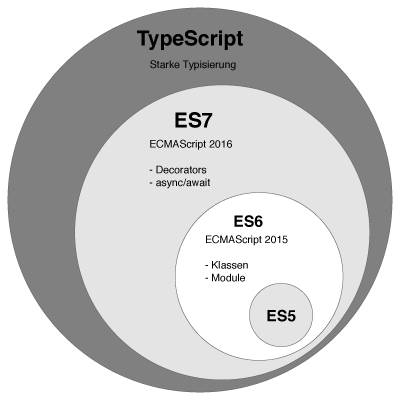
\includegraphics[width=0.5\linewidth]{JavaScript.png}
	\caption{Beziehung zwischen ECMAScript und TypeScript} 
	\quelle{\textcite[28]{Woiwode.2018}}
	\label{fig:ECMAScript}
\end{figure}

\subsection{Die Obermenge TypeScript}
TypeScript ist eine von Anders Hejlsberg bei Microsoft entwickelte Sprache. Diese erweitert die bestehende ECMAScript Version um weitere Sprachelemente und bildet somit eine Obermenge von JavaScript (siehe \autoref{fig:ECMAScript}). Ein Transpilierer übersetzt TypeScript in JavaScript. 

TypeScript ergänzt JavaScript unter anderem um ein stärkeres Typsystem. Hierdurch können Typfehler bereits zur Compilezeit erkannt und Tools zur Codeanalyse (automatische Codevervollständigung, Refactoring-Unterstützung, …) eingesetzt werden.\autocites[vgl.][27\psqq]{Woiwode.2018}[vgl.][13\psqq]{Steyer.2017}[vgl.][10]{Zeigermann.2016} Folgende Basistypen stellt TypeScript zur Verfügung: \autocites[vgl.][34\psqq]{Woiwode.2018}[vgl.][16\psqq]{Steyer.2017}

\begin{itemize}
	\item  \textbf{number}: Ganz- oder Kommazahl
	\item \textbf{string}:  Zeichenkette
	\item \textbf{boolean}: Wahrheitswert
	\item \textbf{Array<typ>}: typisierte Arrays
	\item \textbf{any}: simuliert Standardverhalten von JavaScript  – beliebiger Datentyp
	\item \textbf{Function}: Funktion
\end{itemize}
TypeScript ermöglicht die Verwendung von Interfaces. \autocites[vgl.][40\psq]{Woiwode.2018}

\subsection{Die Erweiterung JSX}
Die Spracherweiterung JSX ermöglicht die Verwendung einer HTML ähnlichen Syntax in JavaScript. JSX wird durch einen geeigneten Transpilierer in gültiges JavaScript übersetzt. 

Die Spracherweiterung kann zum Beispiel bei der Entwicklung mit dem Framework React eingesetzt werden. Dieses Framework verwendet zur Darstellung der Benutzeroberfläche keine Templates. Die Benutzeroberfläche wird stattdessen mit JavaScript Befehlen aufgebaut. Um dies zu erleichtern, kann JSX verwendet werden. Im Folgenden werden die Grundkonzepte von JSX näher erläutert.

Die Ausgabe von dynamische Informationen erfolgt unter Verwendung von JavaScript-Ausdrücken. Diese Ausdrücke müssen in ein paar geschweifter Klammern gepackt werden. Bedingungen können mithilfe des ternären Operatoren überprüft werden. Zur Ausgabe von Listen mit wiederholenden Elementen steht die für Arrays definierte JavaScript Methode map zur Verfügung.

JSX bietet zudem die Möglichkeit das Aussehen eines Elements über das style-Attribut zu verändern. Das sytle-Attribut ist ein Objekt, daher wird die CSS-Eigenschaft und der zugehörige Wert als Objekt-Literal übergeben. Zudem ist zu beachten, dass die CamelCase-Notation für die CSS-Eigenschaften verwendet werden muss. In \autoref{lst:JSXBeispiel} wird die CSS-Eigenschaft \textit{color} und \textit{font-size} des HTML-Elements gesetzt.

Um XSS-Attacken zu verhindern, werden Strings in JSX automatisch escaped bzw. maskiert. Ein String wird demnach immer als Text interpretiert und dargestellt.\autocites[vgl.][59\psqq]{Zeigermann.2016}[vgl.][65\psqq]{Stefanov.2017} 

\begin{lstlisting}[caption=Beispiel für die Verwendung von JSX, label=lst:JSXBeispiel, language=HTML]
const titleColor = 'red';
const titleFontSize = 12;
const helloWorld = <h1 style = {{
	color: titleColor,
	fontSize: titleFontSize + 'px'
	}}> Hello, World</h1>
\end{lstlisting}


\comment{NodeJS}
